\documentclass[journal]{IEEEtran}
\usepackage{graphicx}
\usepackage{url}
\usepackage{amsmath,amssymb}
\usepackage{booktabs}
\usepackage{algorithm}
\usepackage{algpseudocode}
\usepackage{tikz}
\usetikzlibrary{arrows.meta,positioning}
\newtheorem{proposition}{Proposition}
\hyphenation{op-tical net-works semi-conduc-tor Eigen-Score}

\begin{document}

\title{Agreement Meets Confidence: A Training-Free Fusion That Outperforms EigenScore for Hallucination Detection}

\author{Aayaan Ali Khan (202411001), Shlok Bhavsar (202411018), and Prapti Chotaliya (202411030)
\thanks{Course project for CS367, carried out under the guidance of Dr.~Venkata Phanikrishna.}
\thanks{The authors are with the Indian Institute of Information Technology Vadodara -- International Campus Diu, India.}}

\markboth{CS367 Course Project, November 2026}{Khan \MakeLowercase{\textit{et al.}}: Agreement Meets Confidence}

\maketitle

\begin{abstract}
Large language models often state wrong facts with full confidence, and detecting such hallucinations without a reference answer remains difficult. EigenScore, from the INSIDE framework, samples several answers to a question and measures how widely their hidden states spread. We first reproduce EigenScore on an 8 GB consumer GPU. We then show that the same samples carry two further, partly independent kinds of evidence, namely how much the answers agree in their wording and how confident the model is in each token, and we propose a label-free rank fusion of the three signals. Following a development and held-out protocol in which all methods were frozen before the test data were analysed, the fusion outperforms EigenScore by 2.7 points of AUROC on both held-out datasets and by 4.5 points on the development set, with Llama-2-7B on 1,000 questions each from CoQA, TriviaQA and Natural Questions. It is the only method that significantly improves on EigenScore on every dataset, at no additional generation cost.
\end{abstract}

\begin{IEEEkeywords}
Hallucination detection, large language models, rank fusion, uncertainty estimation, internal states.
\end{IEEEkeywords}

\IEEEpeerreviewmaketitle

%=====================================================================
\section{Introduction}
\IEEEPARstart{L}{arge} language models (LLMs) state wrong facts in the same fluent tone as correct ones, so a reader cannot separate the two. A hallucination detector gives each answer a score without access to the correct answer. Existing detectors read one of three kinds of evidence:
\begin{itemize}
\item \textbf{Token confidence} of the generated words, e.g.\ perplexity or length-normalised entropy~\cite{malinin2021}.
\item \textbf{Surface agreement} between several sampled answers, measured on their text~\cite{manakul2023} or meaning~\cite{farquhar2024}.
\item \textbf{Internal states} of the model~\cite{chen2024inside,sriramanan2024}.
\end{itemize}

INSIDE~\cite{chen2024inside} reads internal states. Its \emph{EigenScore} samples $K$ answers and scores the log-volume of their hidden-state embeddings. It therefore sees only one kind of evidence: when the model repeats the same wrong answer $K$ times, the spread collapses and EigenScore trusts it, even though the model's token confidence may still be low.

\textbf{Contributions.}
\begin{enumerate}
\item A working reproduction of INSIDE, whose public code did not run, on an 8~GB laptop GPU.
\item \textbf{TRI}, a training-free rank fusion of internal, surface and token evidence computed from the same samples, together with \textbf{CTC}, a tie-breaking variant with a closed-form gain.
\item A development/held-out evaluation in which every method was committed to version control before the held-out data were analysed. TRI is the only method that significantly beats EigenScore on all three datasets.
\end{enumerate}

%=====================================================================
\section{Related Work}
\textbf{Token-level uncertainty.} Perplexity and length-normalised entropy~\cite{malinin2021} score a single answer from its token probabilities. They are cheap, but a model can be confidently wrong.

\textbf{Sampling consistency.} SelfCheckGPT~\cite{manakul2023} compares sampled answers on their text, and semantic entropy~\cite{farquhar2024} clusters them by meaning before computing an entropy. Both use agreement between samples, but they ignore the model's token confidence and internal states.

\textbf{Internal states.} INSIDE~\cite{chen2024inside} computes a log-determinant over the embeddings of the sampled answers. LLM-Check~\cite{sriramanan2024} applies similar eigen-analysis to the hidden states and attention maps of a single response, and reports that its quality varies across layers. Trained probes on hidden states are accurate but need labelled data~\cite{zhang2025icr}.

\textbf{Evaluation.} Janiak et al.~\cite{janiak2025} show that ROUGE-based labels inflate detector AUROC and that simple baselines are often competitive. This motivates our comparison against strong text baselines and our held-out protocol.

Our work differs from these in combining the three kinds of evidence, without training, from the samples that a sampling-based detector already draws.

%=====================================================================
\section{Existing Work: EigenScore}
For a question, the model samples $K$ answers. Let $\mathbf{z}_k\in\mathbb{R}^d$ be the hidden state of answer $k$'s last token at the middle layer, $Z=[\mathbf{z}_1,\dots,\mathbf{z}_K]$, and $J_d$ the feature-centring matrix. With $\Sigma = Z^\top J_d Z/(d-1)\in\mathbb{R}^{K\times K}$,
\begin{equation}
\mathrm{ES}=\frac{1}{K}\sum_{i=1}^{K}\log_{10}\lambda_i\!\left(\Sigma+\alpha I\right),\qquad \alpha=10^{-3}.
\end{equation}
For a Gaussian, $\tfrac12\log\det\Sigma$ is the differential entropy up to a constant, so ES estimates the semantic uncertainty of the answers~\cite{chen2024inside}.

\textbf{Reproduction.} The released code had twelve blocking defects, among them hard-coded paths, an outdated generation API and a missing dataset loader, and it lacked the feature-clipping component described in the paper. After repairing it, we reproduced the paper's method ranking on 250 CoQA questions with Llama-2-7B in 4-bit precision (Table~\ref{tab:repro}). EigenScore was the best of the five detectors, as in the original paper, although the absolute numbers differ because of quantisation and the smaller sample.

\begin{table}[t]
\centering
\caption{Reproduction of INSIDE on 250 CoQA questions (Llama-2-7B, 4-bit, 8~GB GPU).}
\label{tab:repro}
\footnotesize
\begin{tabular}{@{}lc@{}}
\toprule
Method & AUROC (\%) \\
\midrule
Energy & 54.7 \\
Perplexity & 72.3 \\
LN-Entropy & 77.5 \\
Lexical Similarity & 80.5 \\
\textbf{EigenScore}~\cite{chen2024inside} & \textbf{83.5} \\
\bottomrule
\end{tabular}
\end{table}

\textbf{Two blind spots.} The determinant view explains what EigenScore cannot see. First, if all $K$ answers are identical, their embeddings coincide, $\Sigma\approx 0$ and ES reaches its minimum whether the shared answer is right or wrong. Second, ES never reads the token probabilities that the model computes for every generated word, although these are available at no extra cost.

%=====================================================================
\section{Proposed Method}
\subsection{Three signals from the same samples}
For each question we draw $K=10$ samples and also decode a greedy answer. We compute three scores, each oriented so that a higher value means a more likely hallucination:
\begin{itemize}
\item \textbf{Internal} -- $s_{\mathrm{ES}}$: EigenScore at layer 16.
\item \textbf{Surface} -- $s_{\mathrm{AG}}$: minus the mean pairwise ROUGE-L between the $K$ samples (text agreement).
\item \textbf{Token} -- $s_{\mathrm{TC}}$: LN-Entropy, the mean over samples of the per-token negative log-likelihood.
\end{itemize}
None requires extra generations: the hidden states and log-probabilities are recorded during sampling.

\begin{figure}[t]
\centering
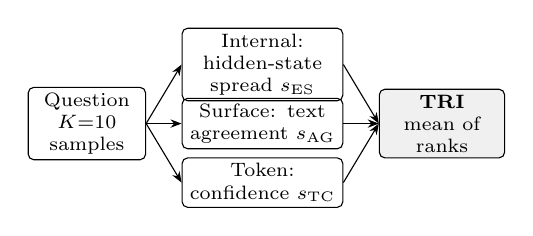
\begin{tikzpicture}[font=\scriptsize, >={Stealth[length=4pt]},
  box/.style={draw, rounded corners=2pt, align=center, minimum height=0.6cm, inner sep=2pt}]
\node[box, text width=1.35cm] (q) {Question\\$K{=}10$ samples};
\node[box, right=0.45cm of q, text width=1.9cm, yshift=0.75cm] (a) {Internal: hidden-state spread $s_{\mathrm{ES}}$};
\node[box, right=0.45cm of q, text width=1.9cm] (b) {Surface: text agreement $s_{\mathrm{AG}}$};
\node[box, right=0.45cm of q, text width=1.9cm, yshift=-0.75cm] (c) {Token: confidence $s_{\mathrm{TC}}$};
\node[box, right=0.45cm of b, text width=1.45cm, fill=black!6] (t) {\textbf{TRI}\\mean of ranks};
\draw[->] (q.east) -- (a.west); \draw[->] (q.east) -- (b.west); \draw[->] (q.east) -- (c.west);
\draw[->] (a.east) -- (t.west); \draw[->] (b.east) -- (t.west); \draw[->] (c.east) -- (t.west);
\end{tikzpicture}
\caption{TRI reads three kinds of evidence from the same $K$ samples and fuses their ranks. No extra generation and no training are needed.}
\label{fig:method}
\end{figure}

\subsection{TRI: rank fusion}
The three scores live on unrelated scales. We therefore fuse their ranks $r(\cdot)$ over the questions:
\begin{equation}
\mathrm{TRI}=\tfrac13\left[r(s_{\mathrm{ES}})+r(s_{\mathrm{AG}})+r(s_{\mathrm{TC}})\right].
\end{equation}
The weights are equal and nothing is fitted, so TRI needs no labels. Ranks are computed over a pool of questions. At deployment, a new answer is ranked against an unlabelled reference pool of earlier questions, i.e.\ each $r(\cdot)$ becomes the empirical CDF of that signal on the pool, so no labels are needed there either. Algorithm~\ref{alg:tri} summarises the procedure.

\begin{algorithm}[t]
\caption{TRI and CTC scoring}
\label{alg:tri}
\footnotesize
\begin{algorithmic}[1]
\Require questions $q_1,\dots,q_N$; model $f$; $K$
\For{$n=1$ to $N$}
  \State sample $a_{n,1},\dots,a_{n,K}\sim f(\cdot\mid q_n)$; keep layer-16 states $\mathbf{z}_{n,k}$ and token log-probs
  \State $s_{\mathrm{ES}}[n]\gets$ EigenScore of $\{\mathbf{z}_{n,k}\}_k$ \Comment{Eq.~(1)}
  \State $s_{\mathrm{AG}}[n]\gets -\frac{2}{K(K-1)}\sum_{k<l}\mathrm{ROUGE\text{-}L}(a_{n,k},a_{n,l})$
  \State $s_{\mathrm{TC}}[n]\gets \frac1K\sum_k \big(-\frac{1}{|a_{n,k}|}\log p(a_{n,k}\mid q_n)\big)$
\EndFor
\State $\mathrm{TRI}\gets\frac13[r(s_{\mathrm{ES}})+r(s_{\mathrm{AG}})+r(s_{\mathrm{TC}})]$
\State $\mathrm{CTC}\gets r_{\text{dense}}(s_{\mathrm{AG}})+\frac{1}{2N}\big(r(s_{\mathrm{TC}})-\tfrac12\big)$
\State \Return TRI, CTC \Comment{higher = more likely hallucination}
\end{algorithmic}
\end{algorithm}

\subsection{CTC: consistency, then confidence}
Text agreement is exactly tied on many questions, mostly where all $K$ samples are identical. AUROC counts a tied correct/incorrect pair as one half: $\mathrm{AUROC}=P(s_1>s_0)+\tfrac12P(s_1=s_0)$. CTC orders questions by $s_{\mathrm{AG}}$ and breaks exact ties by $s_{\mathrm{TC}}$. Every untied pair keeps its order, so the change in AUROC is exactly
\begin{equation}
\Delta\mathrm{AUROC}=(a-\tfrac12)\,P(\text{tied pair}),
\end{equation}
where $a$ is the AUROC of $s_{\mathrm{TC}}$ within the tied pairs.

\begin{proposition}
Let $\mathcal{P}$ be the set of (hallucinated, correct) pairs, $\mathcal{T}\subseteq\mathcal{P}$ the pairs tied under $s_{\mathrm{AG}}$, and $a$ the AUROC of $s_{\mathrm{TC}}$ restricted to $\mathcal{T}$. Then $\mathrm{AUROC}(\mathrm{CTC})-\mathrm{AUROC}(s_{\mathrm{AG}})=(a-\tfrac12)\,|\mathcal{T}|/|\mathcal{P}|$.
\end{proposition}
\begin{IEEEproof}
Dense ranks of distinct values differ by at least 1, while the tie-break term lies in $(0,\tfrac12)$, so CTC preserves the order of every untied pair and those pairs contribute equally to both AUROCs. A tied pair contributes $\tfrac12$ under $s_{\mathrm{AG}}$ and $\mathbb{1}[s_{\mathrm{TC},i}>s_{\mathrm{TC},j}]+\tfrac12\mathbb{1}[s_{\mathrm{TC},i}=s_{\mathrm{TC},j}]$ under CTC. Averaging over $\mathcal{T}$ gives $a$ versus $\tfrac12$; weighting by $|\mathcal{T}|/|\mathcal{P}|$ gives the claim.
\end{IEEEproof}

CTC therefore can only lose if token confidence is worse than chance within ties, and it gains most when ties are frequent. CTC thus targets the self-consistent case that EigenScore misses: when every sample agrees, token confidence is the only evidence left.

%=====================================================================
\section{Experimental Protocol}
\begin{itemize}
\item \textbf{Model.} Llama-2-7B in 4-bit NF4 on an RTX~4060 laptop GPU (8~GB). $K=10$ samples per question at temperature 0.5, top-$p$ 0.99 and top-$k$ 5~\cite{chen2024inside}.
\item \textbf{Data.} 1,000 random questions each from CoQA (story and previous turns in the prompt), TriviaQA (no context) and NQ-Open.
\item \textbf{Feature pass.} Hidden states are read in a second pass that encodes the prompt once and reuses its key--value cache for all $K$ answers, cropping the cache back to the prompt after each answer. Against a full forward pass, the maximum relative difference of the embeddings was $2\times10^{-3}$. All 33 hidden layers are stored as a memory-mapped float16 array, which allows the per-layer analysis below without re-running the model.
\item \textbf{Prompts.} CoQA uses the story and the previous gold question--answer turns; TriviaQA and NQ-Open use a fixed five-shot prompt. Generation stops at a newline, with at most 32 (CoQA) or 20 new tokens.
\item \textbf{Labels.} An answer is a hallucination when its greedy answer has ROUGE-L $\le 0.5$ against every reference.
\item \textbf{Development and held-out split.} All methods were developed on CoQA only. TRI and CTC were then committed to git together with their hypotheses, before any TriviaQA or NQ-Open result was computed.
\item \textbf{Statistics.} AUROC per method; paired bootstrap over questions (10,000 resamples); Holm correction over all held-out superiority tests. A claim counts as confirmed only if it holds on both held-out datasets.
\end{itemize}

%=====================================================================
\section{Results}
\begin{table}[t]
\centering
\caption{AUROC (\%) on 1{,}000 questions per dataset. CoQA was the development set; TriviaQA and NQ-Open were held out.}
\label{tab:auroc}
\small
\setlength{\tabcolsep}{4pt}
\begin{tabular}{@{}lcccc@{}}
\toprule
Method & CoQA & TriviaQA & NQ-Open & Mean \\
\midrule
Perplexity & 74.6 & 79.8 & 74.8 & 76.4 \\
LN-Entropy (token) & 77.8 & 80.6 & 76.0 & 78.1 \\
EigenScore (internal)~\cite{chen2024inside} & 80.1 & 80.5 & 76.7 & 79.1 \\
Text agreement (surface) & 85.3 & 82.5 & 76.6 & 81.5 \\
\midrule
\textbf{CTC} (ours) & \textbf{85.7} & \textbf{83.7} & 77.1 & 82.2 \\
\textbf{TRI} (ours) & 84.6 & 83.2 & \textbf{79.5} & \textbf{82.4} \\
\bottomrule
\end{tabular}
\vspace{2pt}
\footnotesize Model accuracy: CoQA 81.4\%, TriviaQA 69.9\%, NQ-Open 26.9\%.
\end{table}

\begin{table}[t]
\centering
\caption{Held-out confirmation: $\Delta$AUROC (points) with 95\% bootstrap CI. All tests were fixed before the held-out data were analysed.}
\label{tab:held}
\footnotesize
\setlength{\tabcolsep}{2pt}
\begin{tabular}{@{}lccc@{}}
\toprule
Comparison & TriviaQA & NQ-Open & Verdict \\
\midrule
TRI vs EigenScore & +2.7 [+1.7, +3.8] & +2.7 [+1.3, +4.2] & confirmed \\
TRI vs text agreement & +0.7 [$-$0.4, +1.8] & +2.9 [+1.3, +4.5] & non-inferior \\
CTC vs text agreement & +1.2 [+0.6, +1.8] & +0.5 [+0.2, +0.7] & confirmed \\
CTC vs EigenScore & +3.2 [+1.7, +4.8] & +0.3 [$-$1.9, +2.6] & partial \\
Text agreement vs ES & +2.1 [+0.6, +3.5] & $-$0.1 [$-$2.4, +2.2] & partial \\
\bottomrule
\end{tabular}
\end{table}

\textbf{Main result.} Table~\ref{tab:auroc} shows that TRI has the highest mean AUROC, and Table~\ref{tab:held} that it beats EigenScore by 2.7 points on both held-out datasets, significant after Holm correction. On CoQA the gain is 4.5 points (95\% CI $[+2.7,+6.2]$). No single signal is reliable everywhere: text agreement is the strongest signal on CoQA but no better than EigenScore on NQ-Open, where the model answers only 27\% of the questions correctly. There every single signal stays below 77 AUROC, while TRI reaches 79.5.

\begin{figure*}[t]
\centering
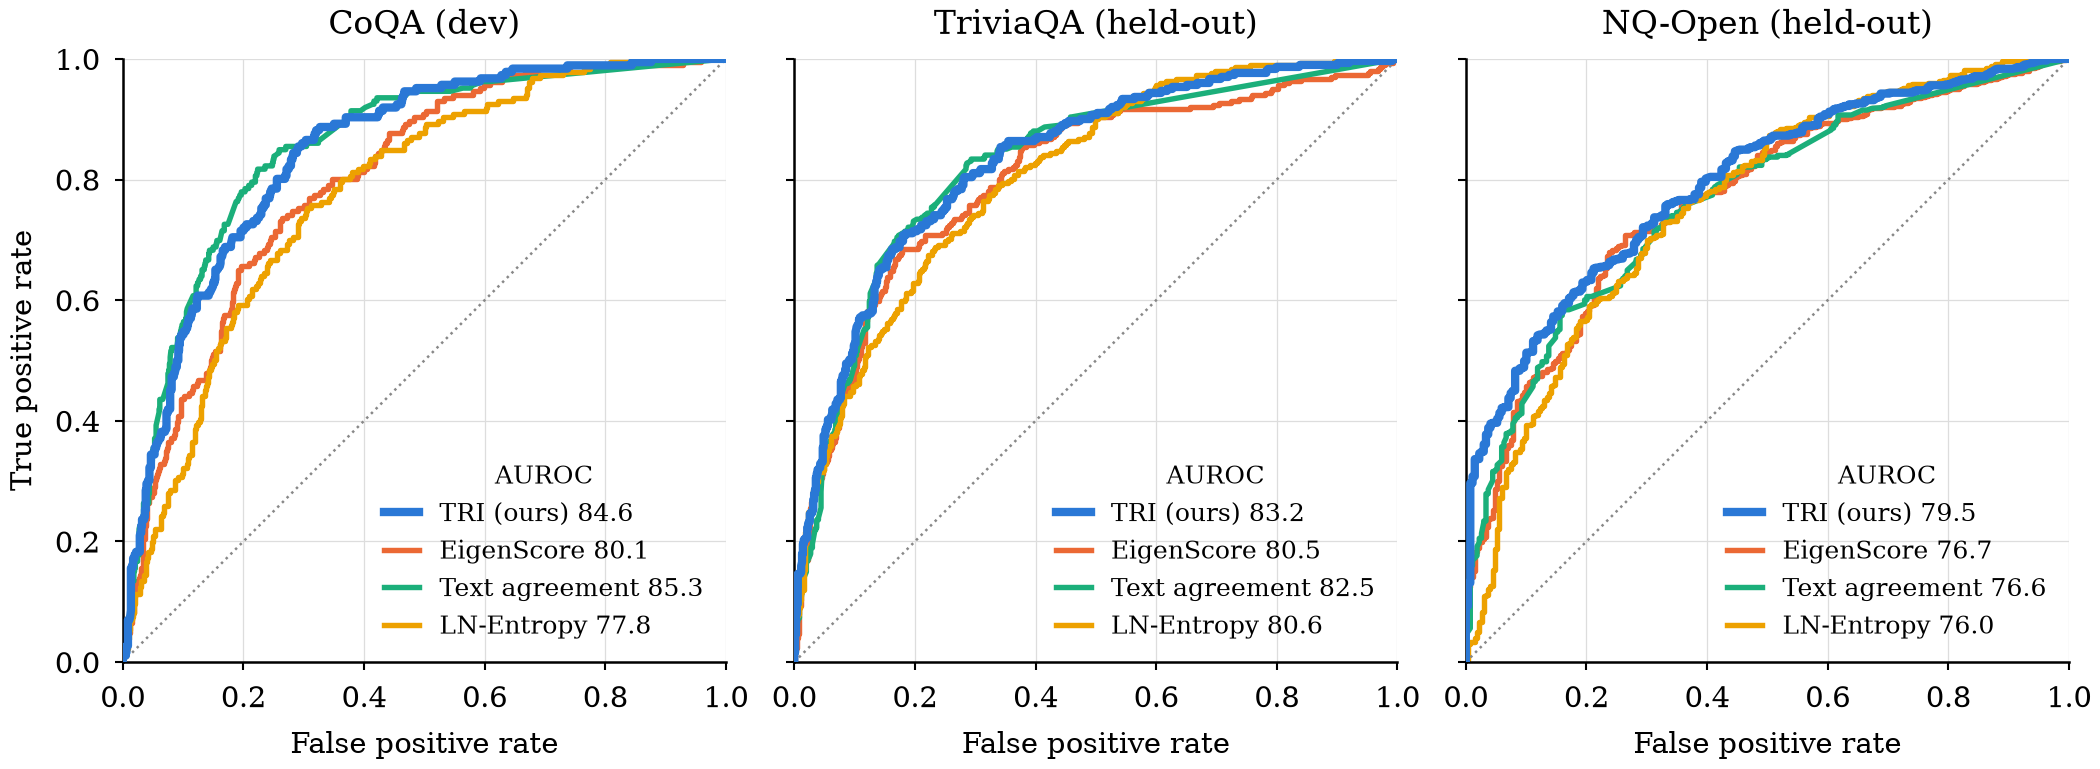
\includegraphics[width=0.92\textwidth]{figures/roc_curves.png}
\caption{ROC curves of TRI and its three input signals. The largest separation appears on NQ-Open at low false positive rates, i.e.\ in the region a deployed detector would operate in, where TRI flags noticeably more hallucinations than any single signal.}
\label{fig:roc}
\end{figure*}

Fig.~\ref{fig:roc} shows the full ROC curves. On the two held-out datasets TRI lies on or above the best single signal over almost the whole range; on NQ-Open its advantage is largest at false positive rates below 0.2.

\textbf{Detection at a fixed false-alarm rate.} AUROC summarises the whole curve, but a deployed detector runs at a fixed, low false positive rate. Table~\ref{tab:tpr} reports the share of hallucinations flagged when only 5\% or 10\% of correct answers may be flagged by mistake. On NQ-Open at 5\%, TRI catches 39.7\% of hallucinations against 28.7\% for EigenScore, i.e.\ 11 more out of every 100. On TriviaQA the gain at 5\% is 4.6 points.

\begin{table}[t]
\centering
\caption{Share of hallucinations flagged (true positive rate, \%) at a fixed false positive rate of 5\% and 10\%.}
\label{tab:tpr}
\footnotesize
\setlength{\tabcolsep}{3.5pt}
\begin{tabular}{@{}lcccccc@{}}
\toprule
 & \multicolumn{2}{c}{CoQA} & \multicolumn{2}{c}{TriviaQA} & \multicolumn{2}{c}{NQ-Open} \\
\cmidrule(lr){2-3}\cmidrule(lr){4-5}\cmidrule(l){6-7}
Method & 5\% & 10\% & 5\% & 10\% & 5\% & 10\% \\
\midrule
LN-Entropy & 19.9 & 32.3 & 32.2 & 45.8 & 18.7 & 37.1 \\
EigenScore & 28.0 & 43.5 & 32.9 & 46.8 & 28.7 & 44.7 \\
Text agreement & \textbf{34.9} & \textbf{55.9} & 34.2 & 49.2 & 31.9 & 43.9 \\
\textbf{TRI} (ours) & 34.4 & 54.3 & \textbf{37.5} & \textbf{52.8} & \textbf{39.7} & \textbf{49.9} \\
\bottomrule
\end{tabular}
\end{table}

\textbf{A self-consistent hallucination.} Asked ``Philopobia is the fear of what basic human emotion?'' (TriviaQA), the model answered ``Fear'' in all ten samples; the correct answer is ``Love''. Because the ten embeddings almost coincide, EigenScore placed this answer at the 2nd percentile of hallucination scores, i.e.\ among the most trusted answers in the dataset. Token confidence placed it at the 81st percentile: the model wrote the same word every time, but with low probability. Similarly, for ``W.~G.~Grace \ldots\ also captained England \ldots\ in what other sport?'', all ten samples read ``Association football'' (correct: lawn bowls); EigenScore ranks it at the 8th percentile and token confidence at the 78th. Across TriviaQA, 25 of the 301 hallucinations (8\%) are of this kind, with ten identical samples; on NQ-Open there are 43. Such cases are invisible to any spread-based score and are exactly where TRI and CTC draw on token confidence.

\textbf{CTC.} CTC beats text agreement on both held-out datasets. Its gains match the closed form of Section~III-C: within tied pairs, token confidence reaches $a=0.73$, $0.70$ and $0.65$ on CoQA, TriviaQA and NQ-Open, on 1.9\%, 5.9\% and 3.1\% of all correct/incorrect pairs. On CoQA, EigenScore reaches only $a=0.59$ within the same ties, which confirms that internal spread carries little information once the answers agree.

\textbf{Why fusion helps.} Rank fusion helps only when the signals err on different questions. Table~\ref{tab:rho} shows that they are only partly correlated. Internal spread and text agreement overlap most ($\rho$ up to 0.90), which is expected since both measure disagreement between the samples, while token confidence is the most independent signal.

\begin{table}[t]
\centering
\caption{Spearman correlation between the three signals.}
\label{tab:rho}
\footnotesize
\begin{tabular}{@{}lccc@{}}
\toprule
Pair & CoQA & TriviaQA & NQ-Open \\
\midrule
Internal -- surface & 0.85 & 0.90 & 0.75 \\
Internal -- token & 0.67 & 0.81 & 0.69 \\
Surface -- token & 0.67 & 0.77 & 0.62 \\
\bottomrule
\end{tabular}
\end{table}

\begin{table}[t]
\centering
\caption{Post-hoc ablation: AUROC of TRI minus AUROC of each two-signal fusion (points, 95\% bootstrap CI). Positive values mean the dropped signal helps.}
\label{tab:ablation}
\footnotesize
\setlength{\tabcolsep}{2.5pt}
\begin{tabular}{@{}lccc@{}}
\toprule
Dropped signal & CoQA & TriviaQA & NQ-Open \\
\midrule
Token & +0.4 [$-$0.7, +1.5] & +1.2 [+0.4, +2.2] & +1.2 [+0.2, +2.2] \\
Surface & +2.5 [+1.6, +3.5] & +1.2 [+0.6, +1.8] & +1.1 [+0.2, +2.0] \\
Internal & +0.0 [$-$0.9, +0.9] & $-$0.6 [$-$1.1, $-$0.0] & +0.6 [$-$0.3, +1.4] \\
\bottomrule
\end{tabular}
\end{table}

The post-hoc ablation in Table~\ref{tab:ablation} agrees. Dropping the surface signal hurts on every dataset, and dropping token confidence hurts on both held-out sets. Dropping the internal signal is neutral on CoQA, slightly helpful on TriviaQA and costs 0.6 points on NQ-Open, where the model is least accurate. The dominant effect is therefore the combination of agreement-type evidence with token confidence; EigenScore adds a small, dataset-dependent contribution, mainly on hard questions. Since this ablation was not pre-registered, we keep the frozen three-signal TRI as our main method.

\textbf{Other pre-registered fusions.} Two further fusions were frozen together with TRI. HYB, the rank sum of a multi-layer EigenScore and token confidence, improved on EigenScore by 1.5 points on both held-out sets, significant on TriviaQA only. PMF, which weighs the samples by their probability and measures the mass that agrees with the greedy answer, reached 83.7 on TriviaQA but did not improve on NQ-Open. Neither is reliable on every dataset, which is why we report TRI and CTC as our methods.

\textbf{Layer choice.} Fig.~\ref{fig:layers} shows single-layer EigenScore at every depth. From layer 5 onward the curve is almost flat, so INSIDE's middle-layer choice is not fragile. Accordingly, averaging EigenScore over layers 8--24 changed AUROC by only $-0.1$ point on every dataset.

\begin{figure}[t]
\centering
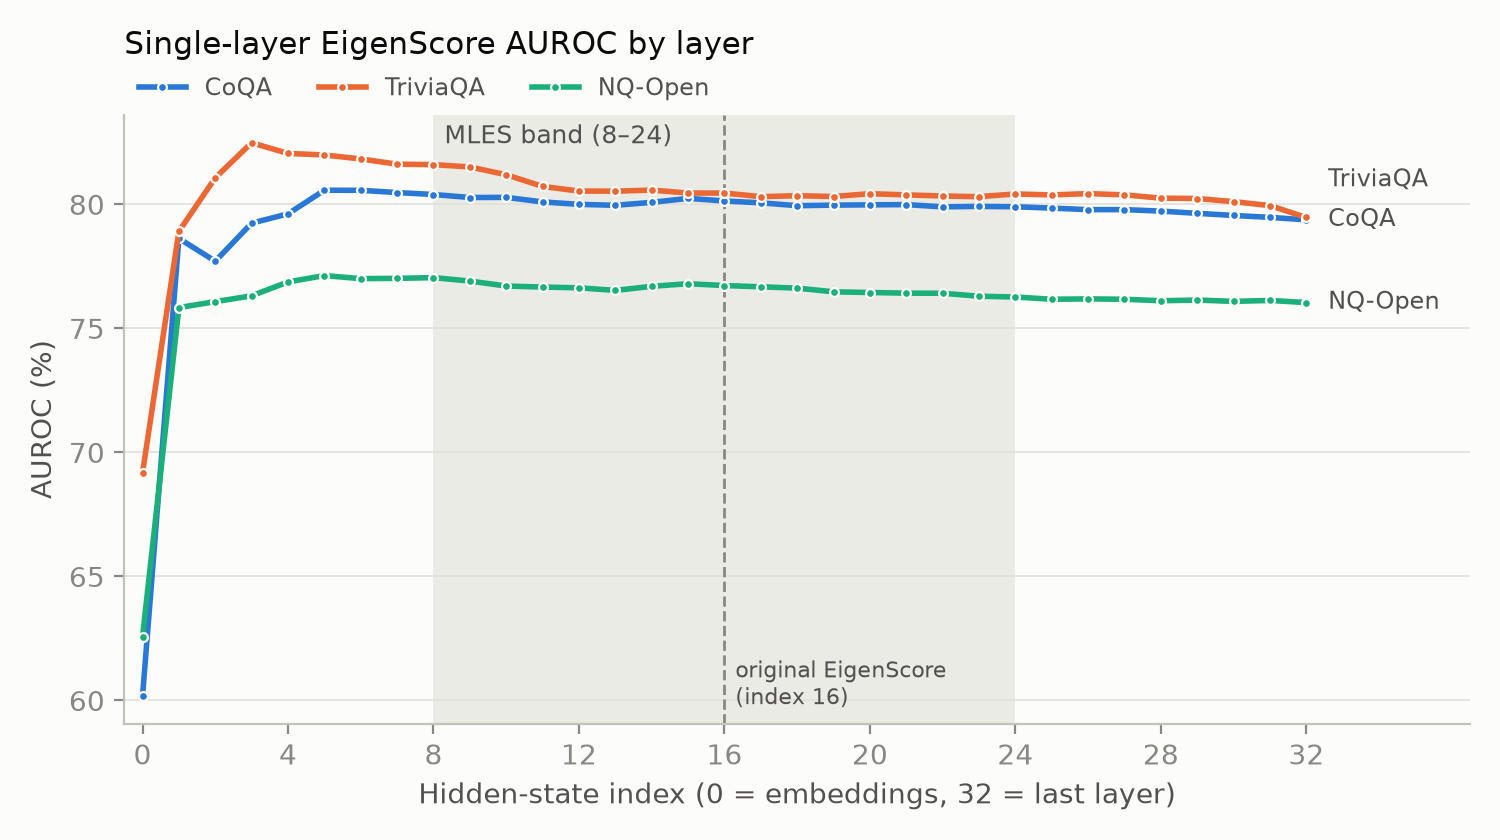
\includegraphics[width=\columnwidth]{figures/per_layer_auroc.png}
\caption{AUROC of single-layer EigenScore at every depth. From layer 5 onward, performance hardly depends on the layer.}
\label{fig:layers}
\end{figure}

\textbf{What did not help.} Before arriving at the fusion, we also tested several EigenScore variants on all three datasets:
\begin{itemize}
\item Multi-layer averaging: $-0.1$ point on every dataset.
\item Normalising the embeddings: between $-0.6$ and $+0.9$ points, not significant.
\item A cross-layer stability score based on representational similarity: $-1.8$ to $-4.3$ points.
\end{itemize}
These results point the same way as the fusion: the gains come from adding a different kind of evidence, not from refining the internal-state signal.

%=====================================================================
\section{Discussion and Limitations}
\begin{itemize}
\item \textbf{Labels.} Correctness is judged by ROUGE-L, which has low precision and inflates the AUROC of sampling-based detectors~\cite{janiak2025}. Paired differences share the same labels and are less affected, but an LLM-judge evaluation is needed.
\item \textbf{Scope.} We study one 7B model in 4-bit precision and 1,000 questions per dataset.
\item \textbf{Cost.} Like EigenScore, TRI needs $K$ generations per question. The fusion itself is free: ranking $N$ questions costs $O(N\log N)$, negligible next to generation.
\item \textbf{Reference pool.} Ranks need a pool of questions. A small unlabelled pool from the same domain suffices, but a strong domain shift between pool and deployment questions would distort the ranks.
\item \textbf{Open-weight models only.} The internal signal requires hidden states. Agreement plus confidence, which carries most of the gain, also works with APIs that expose token log-probabilities.
\end{itemize}

%=====================================================================
\section{Conclusion}
A label-free rank fusion of internal, surface and token evidence, computed from the samples EigenScore already draws, outperforms EigenScore by 2.7 to 4.5 AUROC points on three question-answering datasets. The gains held on two datasets that were frozen out of development. TRI is the only method that significantly improves on EigenScore on every dataset. The main lesson is that confidence and agreement fail on different questions, so a detector should read both. Future work will test a second model family and larger models, replace ROUGE labels with an LLM judge, and study learned but still lightweight fusion weights.

\begin{thebibliography}{10}
\bibitem{chen2024inside} C.~Chen, K.~Liu, Z.~Chen, Y.~Gu, Y.~Wu, M.~Tao, Z.~Fu, and J.~Ye, ``INSIDE: LLMs' internal states retain the power of hallucination detection,'' in \emph{Proc. ICLR}, 2024.
\bibitem{sriramanan2024} G.~Sriramanan, S.~Bharti, V.~S. Sadasivan, S.~Saha, P.~Kattakinda, and S.~Feizi, ``LLM-Check: Investigating detection of hallucinations in large language models,'' in \emph{Proc. NeurIPS}, 2024.
\bibitem{farquhar2024} S.~Farquhar, J.~Kossen, L.~Kuhn, and Y.~Gal, ``Detecting hallucinations in large language models using semantic entropy,'' \emph{Nature}, vol.~630, pp.~625--630, 2024.
\bibitem{manakul2023} P.~Manakul, A.~Liusie, and M.~J.~F. Gales, ``SelfCheckGPT: Zero-resource black-box hallucination detection for generative large language models,'' in \emph{Proc. EMNLP}, 2023.
\bibitem{malinin2021} A.~Malinin and M.~Gales, ``Uncertainty estimation in autoregressive structured prediction,'' in \emph{Proc. ICLR}, 2021.
\bibitem{zhang2025icr} Z.~Zhang \emph{et al.}, ``ICR Probe: Tracking hidden state dynamics for reliable hallucination detection in LLMs,'' in \emph{Proc. ACL}, 2025.
\bibitem{janiak2025} D.~Janiak, J.~Binkowski, A.~Sawczyn, B.~Gabrys, R.~Shwartz-Ziv, and T.~Kajdanowicz, ``The illusion of progress: Re-evaluating hallucination detection in LLMs,'' arXiv:2508.08285, 2025.
\end{thebibliography}

\end{document}
